\chapter{Baseline Motion System} \label{chap:motion}
    This chapter covers the systems governing the baseline motion of the robot, meaning the motion over simple flat terrain. First the kinematics of the robot are modelled, Next the walking gait state machine is described. And finally, the equations to define a foot's path of motion is described. An overview of these systems can be seen in figure \ref{fig:motion_system}.
    \begin{figure}[h]
        \centering
        % \hspace{-1.38cm}
        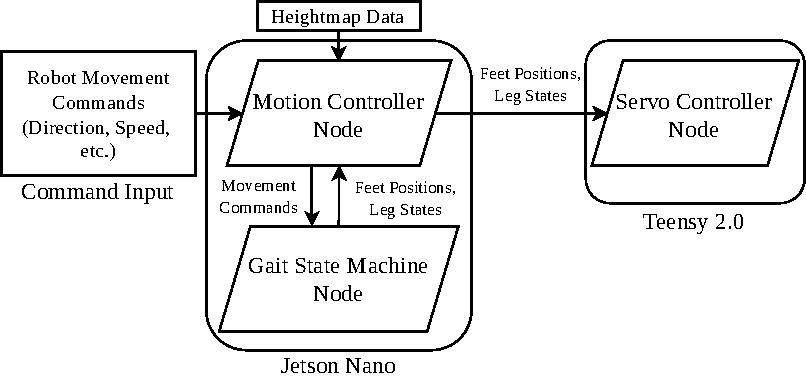
\includegraphics{Diagrams-MotionSystem.drawio.pdf}
        \caption{Motion System Overview}
        \label{fig:motion_system}
    \end{figure}
    \section{Overview}
        % This chapter describes the systems governing the motion of the robot, such as leg motion planning and gait generation.
        The basic operation of the motion system is as follows: First the robot is commanded to walk in a certain direction, at a certain speed, and with a certain body height. These commands are sent from the base station to the Jetson Nano on the robot. The motion controller node on the Jetson Nano then sends these commands to the gait state machine node, at a fixed frequency. The gait state machine uses the received direction and stride length to generate leg states (swinging or supporting) and the ideal final position of each foot. These states and positions are sent back to the motion controller node where the positions are adjusted based on the heightmap data to ensure stable footing. The leg states and adjusted feet positions are then sent to the servo controller node. This node controls the servos to move the robot's feet to their final positions, either in a arc or linearly, depending on their state (swinging or supporting). %A high level diagram of the motion system can be seen in \ref{fig:motion_system}.

    \section{Kinematics}
        When commanding a foot position, the servo controller requires a function to calculate servo angles. While the foot arc planner, which will be described in section \ref{sec:arc_generation}, requires the current position of the feet to function. The inverse and forward kinematic functions described in this section provide this functionality. 
        
        \subsection{Coordinate Frames}
            The coordinate frames relevant to the kinematics of the robot are the body coordinate frame, \fbody, and the leg frames, \fleg. All foot targets/positions are specified in the body coordinate frame, while the kinematic systems operate in the leg coordinate frames. Thus conversions from the body to leg frames are required. Figure \ref{fig:coords_top} shows the world, body, and leg coordinate frames.
            \begin{figure}[h]
                \centering
                % \hspace{-1.38cm}
                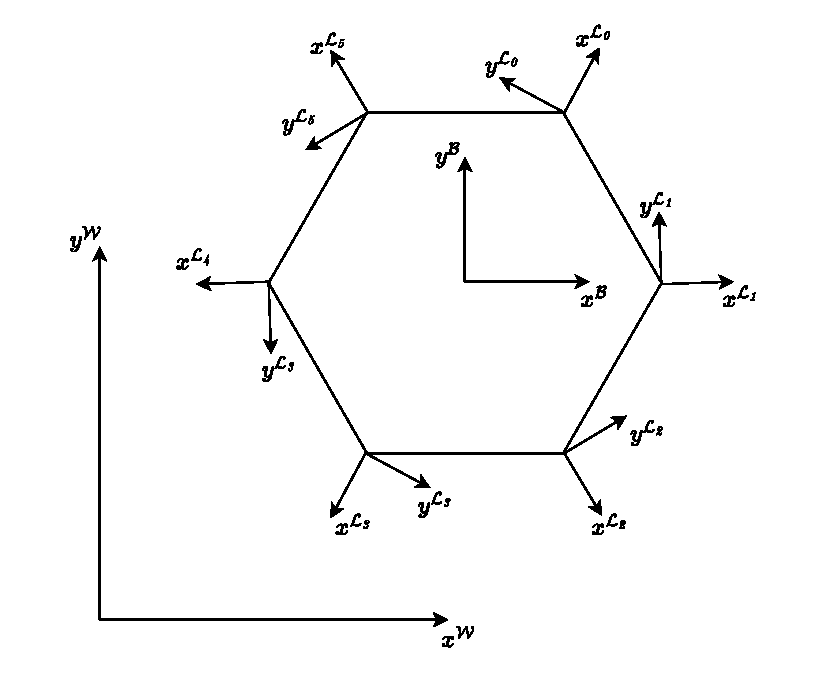
\includegraphics[width=.68\textwidth]{Diagrams-BodyFrame.drawio.pdf}
                \caption{World, body and leg coordinate frames.}
                \label{fig:coords_top}
            \end{figure}

            \noindent
            The leg coordinate systems are simply rotated and shifted from the body coordinate system. This transformation,\transframe{\bm{x}^\fbody}{\fbody}{\fleg} is defined by equation \ref{eq:body_to_leg}, further explained in appendix \ref{app:transforms}.
            \begin{equation}\label{eq:body_to_leg}
            \begin{split}
                \bm{x}^\fleg &= \transframe{\bm{x}^\fbody}{\fbody}{\fleg} \\
                & = \bm{Q}_i^\fbody\cdot\bm{x}^\fbody\cdot\bm{Q}^{\fbody^{-1}}_{i} - \bm{R}_i
            \end{split}
            \end{equation}

            \noindent
            where \(\fleg\) is the coordinate frame of leg \(i\), \(\bm{Q}_i^\fbody\) is the rotation of said coordinate frame and \(\bm{R}^\fbody_i\) is the root position of said leg coordinate frame in the body coordinate frame. For more detail on this transformation, such as the values of \(\bm{Q}_i^\fbody\) and \(\bm{R}^\fbody_i\), please see
            appendix \ref{app:transforms}.

            Now that positions can be transformed into the leg coordinate frames, the kinematic equations, as described in the following sections, can be applied. The kinematic equations are defined with reference to the variables in the leg frame as shown in figure \ref{fig:kinematics}.
            \begin{figure}[h]
                \centering
                % \hspace{-1.38cm}
                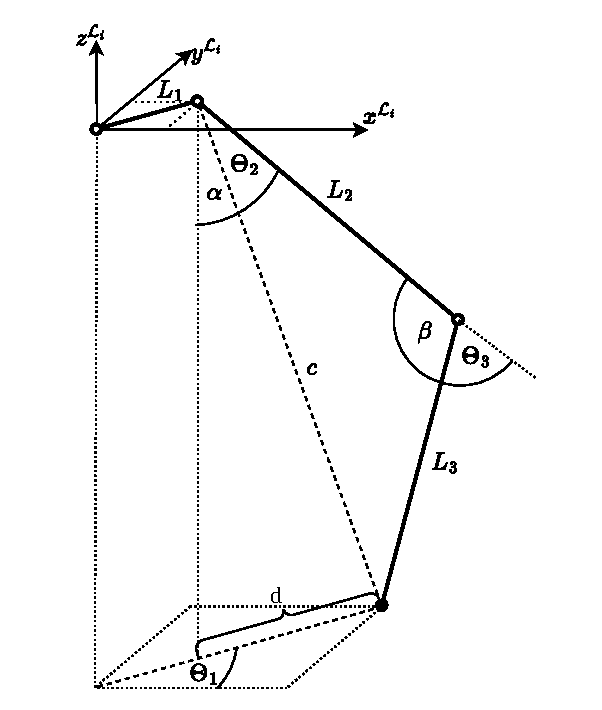
\includegraphics[clip, trim=0 0 1.1cm 0]{Diagrams-Kinematics.drawio.pdf}
                \caption{Leg coordinate frame with kinematic variables.}
                \label{fig:kinematics}
            \end{figure}

        \newpage
        \subsection{Inverse Kinematics}
            The inverse kinematic function calculates the leg servo angles, \(\bm{\Theta}\inrefframe{\fleg} = [\Theta_1, \Theta_2, \Theta_3]^T_{\displaystyle ,}\) required for the foot to be at the given target position vector, \(\bm{t}\inrefframe{\fleg} = [x_t,y_t,z_t]^T_{\displaystyle .}\) The inverse kinematic equations are described by
            \begin{equation}\label{eq:ik}
                \bm{\Theta}\inrefframe{\fleg}(x_t,y_t,z_t) =
                                    % \begin{bmatrix}
                                    %     \Theta_1\\
                                    %     \Theta_2\\
                                    %     \Theta_3
                                    % \end{bmatrix}
                                    % =
                                    \begin{bmatrix}
                                        \arctan{\left(\dfrac{x_t}{y_t}\right)}\\[0.5cm]
                                        \dfrac{\pi}{4} - \alpha - \arctan{\left(\dfrac{y_t}{d-L_1}\right)}\\[0.5cm]
                                        \dfrac{\pi}{2} - \beta
                                    \end{bmatrix}
            \end{equation}
            where \(\alpha\), \(\beta\), \(c\) and \(d\) are calculate as follows:
            \begin{align}
                \alpha &= \arcsin{\left(\frac{L_3\sin{\beta}}{c}\right)} \label{eq:alpha} \\[0.5cm]
                \beta &= \arccos{\left(\dfrac{L_1^2 + L_2^2 -c^2}{2L_1L_2}\right)}\\[0.5cm]
                c &= \sqrt{(d-L_1)^2+z_t^2}\\[0.5cm]
                d &= \sqrt{x_t^2 + y_t^2} \label{eq:dik}
            \end{align}
        \subsection{Forward Kinematics}
            The forward kinematics function calculates the position vector of a foot, \(\bm{p}_f\inrefframe{\fleg} = [x_f,y_f,z_f]^T\), given the current angles of the leg servos, \(\bm{\theta}\inrefframe{\fleg} = [\theta_1, \theta_2, \theta_3]^T\).
            \begin{align}
                \bm{p}_f\inrefframe{\fleg}(\theta_1,\theta_2,\theta_3) =
                                % \begin{bmatrix}
                                %     x_c\\
                                %     y_c\\
                                %     z_c
                                % \end{bmatrix}
                                % =
                                \begin{bmatrix}
                                    d\cos{\theta_1}\\
                                    d\sin{\theta_1}\\
                                    L_2\sin{\theta_2} + L_3\sin{\left(\theta_2 + \theta_3\right)}
                                \end{bmatrix}
            \end{align}
            where \(d\) is calculated as follows:
            \begin{equation}\label{eq:dfk}
                d = L1 + L_2\sin{\theta_2} + L_3\sin{(\theta_2 + \theta_3)}
            \end{equation}
        
        \newpage
        \subsection{Angular Rate} \label{sec:ang_rate}
            To move a foot on a desired path it is important to not only know the absolute angle of the three leg servos, but also the angular rates of all three
            servos. If the servos are all moved at the same rate, the shape of the path that the foot follows will not be linear, but rather dependant on the
            current foot position. This is undesirable, thus equations \ref{eq:rate} defines the derivative of the inverse kinematics equations (\ref{eq:ik}), i.e. the angular
            rate, given the target movement speeds of a foot, \(\dot{x}\), \(\dot{y}\) and \(\dot{z}\).

            \begin{equation}\label{eq:rate}
                \bm{\omega}(\dot{x}, \dot{y}, \dot{z}) =
                                    % \begin{bmatrix}
                                    %     \omega_1\\
                                    %     \omega_2\\
                                    %     \omega_3
                                    % \end{bmatrix}
                                    % =
                                    \begin{bmatrix}
                                        \dfrac{- x\dot{y} + y \dot{x}}{x^2 + y^2}\\[0.5cm]
                                        \dfrac{\left[(L_1 - d)\dot{z} + z\dot{d}\right]\alpha + \Big[(L_1 - d)^2 + z^2\Big]\arctan{\left(\dfrac{L_1-d}{z}\right)}\dot{\alpha}}{(L_1 - d)^2 + z^2}\\[0.8cm]
                                        -\dot{\beta} 
                                    \end{bmatrix}
            \end{equation}
            where \(\dot\alpha\), \(\dot\beta\), \(\dot{c}\) and \(\dot{d}\) as shown in equations \ref{eq:alphadot} to \ref{eq:cdot}.
            \begin{align}
                \dot{\alpha} &= \frac{ L_3\left[ c\cos(\beta)\dot{\beta} - \sin(\beta)\dot{c} \right] }{ c^2\sqrt{-\dfrac{L_3^2\sin^2(\beta)}{c^2}+1} } \label{eq:alphadot} \\[0.5cm] 
                \dot{\beta} &= \frac{ 2c\dot{c} }{ L_2L_3\sqrt{4 - \dfrac{(L_2^2+L_3^2-c^2)^2}{L_2^2L_3^2}} } \label{eq:betadot} \\[0.5cm]
                \dot{c} &= \frac{-(L_1 - d)\dot{d} + z\dot{z}}{\sqrt{(L_1 - d)^2 + z^2}} \label{eq:bdot} \\[0.5cm]
                \dot{d} &= \frac{x\dot{x} + y\dot{y}}{\sqrt{x^2 + y^2}} \label{eq:cdot}
            \end{align}
    
    \newpage
    \section{Walking Gait}
        To move, the hexapod must support its body with some of its legs while the remaining legs swing towards their new targets, at which point the swinging legs become the new supporting legs. The sequence in which the legs support and swing is called the walking gait. Figure \ref{fig:gait_patterns} shows three different gait patterns that can be used with a hexapod, namely the wave, ripple, and tripod gaits \citep{Darbha2017AnOS}. A dark cell represents a swinging leg and a light cell a supporting leg.
        \begin{figure}[h]
            \centering
            % \hspace{-1.38cm}
            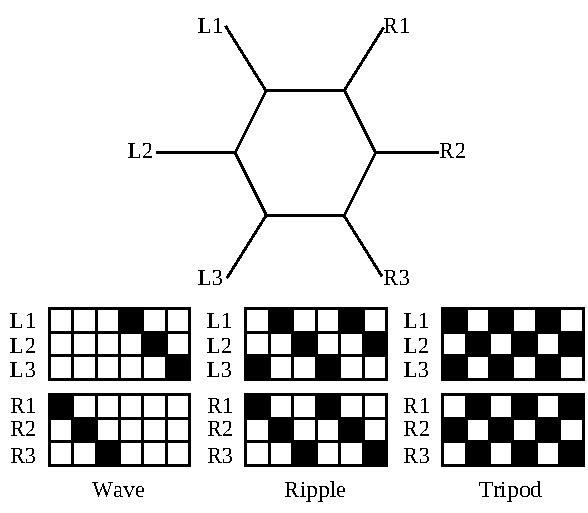
\includegraphics{Diagrams-GaitDiagram.drawio.pdf}
            \caption{Three hexapod gait patterns.}
            \label{fig:gait_patterns}
        \end{figure}

        \noindent
        The wave gait moves one leg at a time while supporting with the remaining 5, the ripple gait moves two legs at a time, and the tripod moves three legs at a time.

        The speed of the hexapod is based on the parameters of the gait, specifically as described in equation \ref{eq:speed},
        \begin{equation} \label{eq:speed}
            v = \frac{S}{D\tau}
        \end{equation}
        where \(S\) is the stride length, \(\tau\) is the gait period and \(D\) is the duty factor. \(D\) is defined as the time a leg is in the support phase relative to its swing phase. The wave, ripple and tripod gaits have duty factors of \(\frac{5}{6}\), \(\frac{2}{3}\) and \(\frac{1}{2}\) respectively.
        
        From this it is clear that the wave gait is the slowest while the tripod gait is the fastest, and the ripple gait is in-between. It should however be noted the gait's stability is inverse to their speed.

        The gait that will be used in this system is the tripod gait, which is the most common gait for hexapods as it supports with three legs, while maximising speed. Even though this is less stable than
        the wave and ripple gaits, it does maintain natural stability with three contact points, which is adequate for most circumstances.

        \subsection{Stride Reference Frame}
            When describing the stride of the robot it is important to note which reference frame is being used. Figure \ref{fig:stride_body} shows
            the stride of a tripod gait in the body reference frame, \(\fbody\).
            \begin{figure}[h]
                \centering
                % \hspace{-1.38cm}
                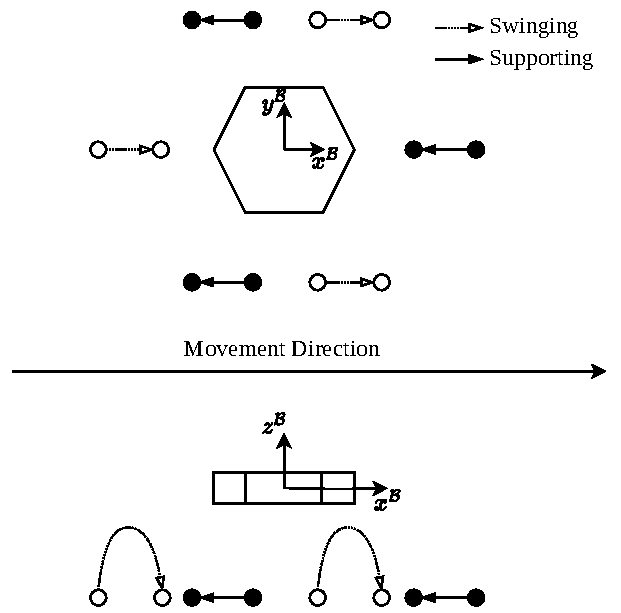
\includegraphics{Diagrams-StrideDiagramLocal.drawio.pdf}
                \caption{Hexapod stride relative to body coordinates.}
                \label{fig:stride_body}
            \end{figure}

            \noindent
            As can be seen, the swinging legs move in the direction of movement, following an arced path, while the supporting legs move in the opposite direction of movement following a linear path. 

            \newpage
            \noindent
            However, when looking at the same stride in the world reference frame, \(\fworld\), as can be seen in figure \ref{fig:stride_world},
            the supporting legs appear to stay stationary, while the swinging legs move double the distance relative to that in the body reference frame.
            \begin{figure}[h]
                \centering
                % \hspace{-1.38cm}
                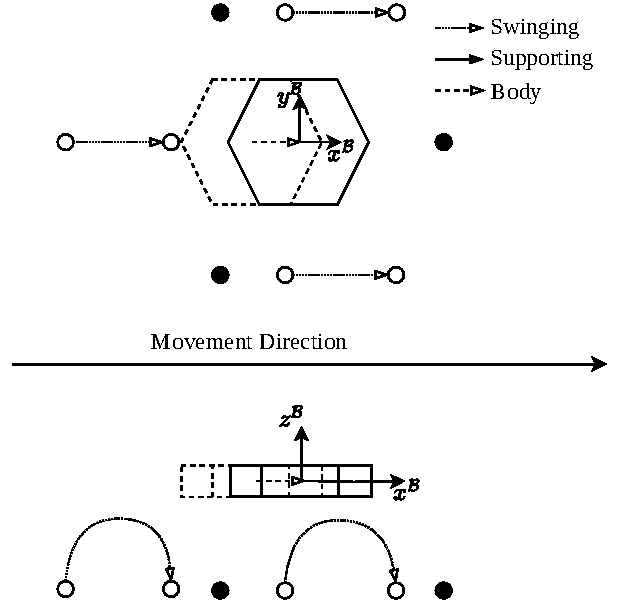
\includegraphics{Diagrams-StrideDiagramGlobal.drawio.pdf}
                \caption{Hexapod stride relative to world coordinates.}
                \label{fig:stride_world}
            \end{figure}

            \noindent
            This is important to note because, as further discussed in section \ref{sec:choosing_nominal}, the nominal foot positions are chosen in the body reference frame, but must target a
            position in the world reference frame.
        
        \newpage
        \subsection{State Machine}
            The state machine used to realise the tripod gait used in the robot is quite simple, comprised of only two states, namely stepping and
            resting, as can be seen from figure \ref{fig:gaitSM}. Table \ref{tab:state_defs} defines the actions that should be taken during
            each state.

            The primary computation done by this state machine is calculating which legs are supporting and which are swinging, which occurs
            on entering the "Stepping" state. This function is described in section \ref{sec:supp_swing_calc}.

            \begin{figure}[h]
                \centering
                % \hspace{-1.38cm}
                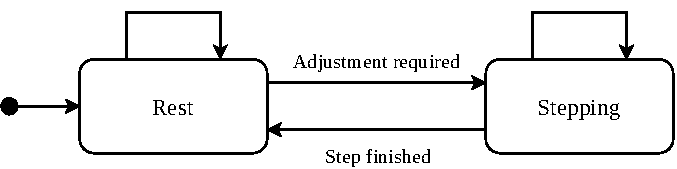
\includegraphics{Diagrams-GaitSM.drawio.pdf}
                \caption{Gait State Machine}
                \label{fig:gaitSM}
            \end{figure}

            \begin{table}[h]
                \center
                \begin{tabularx}{\textwidth}{|l|X|}
                    \hline
                    \multicolumn{2}{|c|}{Rest State Definition} \\
                    \hline
                    Enter Condition & Has all feet reached their targets? \\
                    \hline
                    On Entering & Set all leg states as supporting. \\
                    \hline
                    While Active & Do nothing \\
                    \hline
                \end{tabularx}
                
                \bigskip
                \noindent
                \begin{tabularx}{\textwidth}{|l|X|}
                    \hline
                    \multicolumn{2}{|c|}{Stepping State Definition} \\
                    \hline
                    Enter Condition & Is there a mismatch between feet targets and current position? \\
                    \hline
                    On Entering & Calculate and set the leg states based on walking direction, see section \ref{sec:supp_swing_calc}. Choose and optimise nominal targets
                    for the current step, see chapter \ref{chap:optimisation}\\
                    \hline
                    While Active & Adjust feet targets based on direction, stride length and robot height, see chapter \ref{chap:optimisation}\\
                    \hline
                \end{tabularx}
                \caption{State Definitions}
                \label{tab:state_defs}
            \end{table}

        \newpage
        \subsection{Choosing the Supporting and Swinging Legs} \label{sec:supp_swing_calc}
            The robot body is divided up into sextants, centered around the nominal leg positions. When calculating
            the swinging legs it is first determined in which sextant the movement direction vector falls, this is called the active sextant.
            The leg related with the active sextant, and the two opposite, are then chosen as swinging, with the remaining three legs chosen as supporting.
            The states of the legs stored in a boolean array.
            % \begin{equation}\label{eq:is_swing}
            %     \bm{S}_{\bm{i} - \xi}=[i \text{ is even}]
            % \end{equation}
            % where \(\xi \in i\) is the active sextant/leg number, and,
            % \[i = \seq{0}{1}{5}\]
            Figure \ref{fig:sextants} illustrates and example with sextant 1 being active. Thus legs 1, 3 and 5 are swinging, while legs 0, 2 and 4 are supporting.
            \begin{figure}[h]
                \centering
                \hspace{1.1cm}
                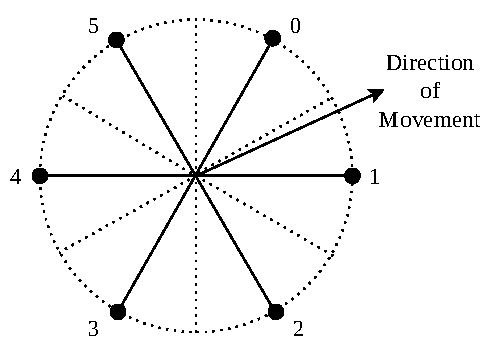
\includegraphics[clip, trim=0 0.25cm 0 0.25cm]{Diagrams-Sextants.drawio.pdf}
                \caption{Leg sextants, with sextant 1 currently being active.} 
                \label{fig:sextants}
            \end{figure}
            
            \noindent
            This of course would not be sufficient to define a walking gait, as at the end of each step the boolean array containing the leg states needs to be inverted. Thus, at the end of each step, if the currently swinging legs are the same as those in the previous step, then the boolean array is inverted.
            
            % and additional step after equation \ref{eq:is_swing} is added. The current horizontal length of leg \(\xi\), defined as \(l_\xi\), is compared to its nominal horizontal length, \(L_\xi\). If \(l_\xi\ > L_\xi\), invert \(\bm{S_i}\).
            % \begin{equation} \label{eq:negate_is_swing}
            %     \bm{S}_{\bm{i} - \xi} =
            %                                         \begin{cases}
            %                                             \bm{i} \setminus \bm{S}_{\bm{i} - \xi} & l_\xi > L_\xi \\
            %                                             \bm{S}_{\bm{i} - \xi} & l_\xi \leq L_\xi
            %                                         \end{cases}\\[0.1cm]
            % \end{equation}

        \subsection{Choosing nominal foot positions}\label{sec:choosing_nominal} 
            Once the active and inactive legs have been selected, it is required to choose nominal targets for all the feet. Sections \ref{sec:support} and \ref{sec:swing}
            describe the process for finding the support and swinging leg target positions. It should be noted that target matrices, denoted by \(\bm{t}\), are common between these two sections, but are computed differently depending on whether the leg is swinging or supporting.
                
            \subsubsection{For Supporting Legs} \label{sec:support}
                The supporting leg nominal targets are chosen by first calculating the move vector \(\boldsymbol{m}^\fbody\), and then adding the move vector to the foot's target position in it's swinging phase, which should be equal to the foot's current position. The move vector is calculated as the vector from the foot's nominal target, from the foot's swinging phase, to the movement direction, \(\bm{w}_\text{dir}^\fbody\), inverted, multiplied by the stride length, and added to the foot's constant resting position, \(\bm{T}^\fbody\). \(\bm{T}^\fbody\) is  a constant that contains the positions of the feet when the robot is standing still, on flat terrain.
                Equations \ref{eq:move_vec} and \ref{eq:opt_supp} describe this process, with reference to figure \ref{fig:supp_targ}.
                \begin{figure}[h]
                    \centering
                    % \hspace{1.1cm}
                    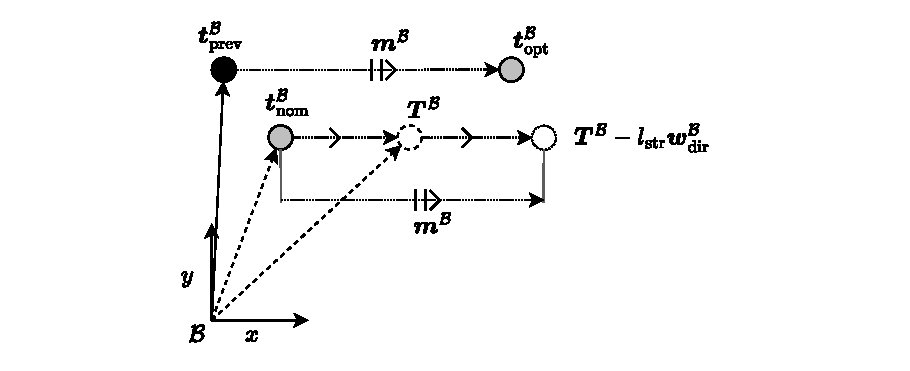
\includegraphics[clip, trim=3cm 0.25cm 3.4cm 0.25cm]{Diagrams-ChooseNominalSupp.drawio.pdf}
                    \caption{Supporting target choosing diagram in the body frame.} 
                    \label{fig:supp_targ}
                \end{figure}

                \noindent
                First the required move vectors, \(\bm{m} ^\fbody\), are calculated in equation \ref{eq:move_vec},
                \begin{equation}\label{eq:move_vec}
                    \mdim{\boldsymbol{m}^\fbody}{3}{1} =  (\bm{T}^\fbody - l_\text{str} \bm{\bm{w}_\text{dir}}^\fbody) - \bm{t_\text{nom}}^\fbody
                \end{equation}
                where \(\bm{T}^\fbody\) contains the constant resting positions of the feet, \(l_\text{str}\) is the nominal stride length, \(\bm{w}_\text{dir}^\fbody\)
                contains the desired walk directions, and \(\bm{t}_\text{nom} ^\fbody\) contains the nominal targets as calculated in
                equation \ref{eq:swing_nom}.

                Then the optimised targets, \(\bm{t_\text{opt}} ^\fbody\), are calculated as the addition of the previous targets and the move vector in equation \ref{eq:move_vec},
                \begin{equation} \label{eq:opt_supp}
                    \mdim{\boldsymbol{t}_\text{opt}^\fbody}{3}{6} = \bm{t}_\text{prv}^\fbody + \bm{m}^\fbody
                \end{equation}
                where \(\bm{t}_\text{prv}^\fbody\) contains the previous, optimised, targets. Note that equation \ref{eq:opt_supp} does not include the optimisation
                function, described in chapter \ref{chap:optimisation}. This is because the supporting feet will not move relative to the terrain, and thus do not need their targets optimised.
            
            \newpage
            \subsubsection{For Swinging Legs} \label{sec:swing}
                The swinging leg nominal targets are chosen by adding the movement, direction, \(\bm{w}_\text{dir}^\fbody\), multiplied by the stride length, to the constant feet resting positions, \(\bm{T}^\fbody\), and the movement vector of the supporting legs, \(\bm{m} ^\fbody\).
                
                A diagram of this process is shown in figure \ref{fig:swinging_targ}. Please note that \(\bm{t}_\text{nom}^{\fmap}\) is in map space, thus \(\bm{t}_\text{nom}^{\fmap}\) is represented as \(\transframe{\bm{t}_\text{nom}^{\fmap}}{\fmap}{\fbody}\) in the figure, because the figure is in body space. This map to body transform is purely for illustrative purposes and is not used in the actual system, as it simply reverses the body to map transform in equation \ref{eq:t_map}.
                \begin{figure}[h]
                    \centering
                    % \hspace{1.1cm}
                    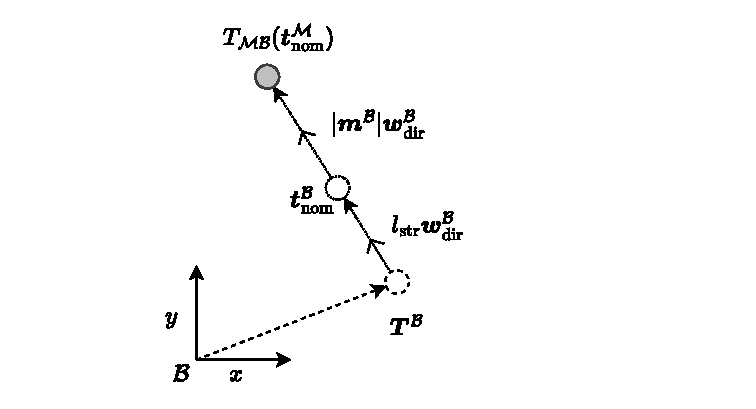
\includegraphics[clip, trim=2.5cm 0.25cm 4.9cm 0.3cm]{Diagrams-ChooseNominalSwing.drawio.pdf}
                    \caption{Swinging target choosing diagram in the body frame.} 
                    \label{fig:swinging_targ}
                \end{figure}

                \noindent
                The swinging nominal targets, in map space, \(\bm{t_\text{nom}} ^{\fmap}\), are calculated as follows,
                \begin{equation} \label{eq:t_map}
                    \mdim{\boldsymbol{t}_\text{nom}^{\fmap}}{3}{6} = \transframe{\bm{T}^\fbody + \left(l_\text{str}+\bm{m}^\fbody\right)\bm{w}_{dir}^\fbody}{\fbody}{\fmap}
                \end{equation}
                where \(\bm{T}^\fbody\) contains the constant rest positions the feet, \(l_\text{str}\) is the nominal stride length, \(\bm{w}_\text{dir}^\fbody\) contains the desired walk directions. \(\bm{m}^\fbody\) is the average move vector.

                For use in equation \ref{eq:move_vec}, the swinging legs nominal targets, \(\bm{t_\text{nom}} ^\fbody\), are calculated as 
                in equation \ref{eq:swing_nom},
                \begin{equation} \label{eq:swing_nom}
                    \mdim{\boldsymbol{t}_\text{nom}^\fbody}{3}{6} = \bm{T}^\fbody + l_{str}\bm{w}_\text{dir}^\fbody
                \end{equation}

                \noindent
                Note that \(\transframe{\bm{t}_\text{nom}^{\fmap}}{\fmap}{\fbody}\) is quite similar to \(\bm{t}_\text{nom}^\fbody\), the difference is that \(\bm{t}_\text{nom}^{\fmap}\) is set such that it will align with \(\bm{t}_\text{nom}^\fbody\) at the end of the step. Explaining the omission of the support phase move vector, \(\bm{m}^\fbody\), in calculating \(\bm{t}_\text{nom}^\fbody\) in equation \ref{eq:swing_nom}. Meaning that until the end of the step, \(\bm{t}_\text{nom}\inrefframe{M}\) and \(\bm{t}_\text{nom}^\fbody\) will point to different positions in world space. This is due to needing to account for body movement in map space, but not in local space.

        \newpage
    \section{Trajectory Generation} \label{sec:arc_generation}
        When taking a step, the foot can not simply be moved to its destination in a straight line, as doing so will cause the foot to be dragged on the terrain, impeding the movement of the robot. Thus it is required to move the foot in an arc-like trajectory to clear any obstacles that might be in its path.

        A new method of generating trajectories is described in section \ref{sec:imporved}, as opposed to the existing system by \cite{erasmus2023guidance}, which is described in section \ref{sec:existing}.

        \subsection{Existing Trajectory System} \label{sec:existing}
            The existing system will, at the start of each step, compute an arc for each foot to follow, this arc is then sent to the servo controller
            to be executed. The arc is computed as a polynomial passing through three points, the initial point\(q_i\), the midpoint \(q_m\), and the final point \(q_f\).
            Figure \ref{fig:old_arc_vars} shows the variables used to calculate this arc.
            \begin{figure}[h]
                \centering
                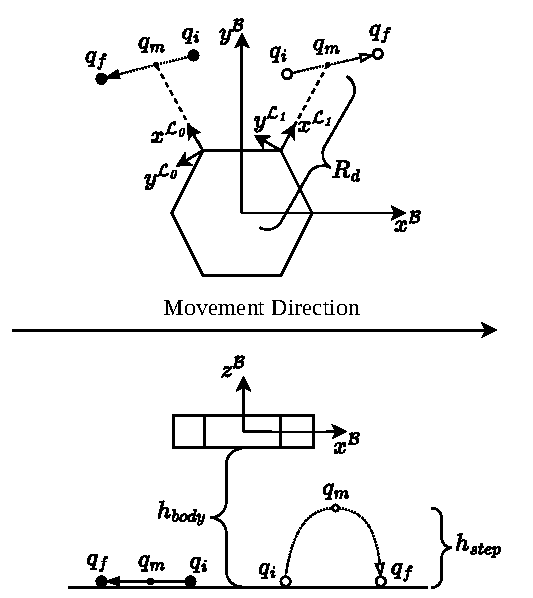
\includegraphics{Diagrams-ArcCalc.drawio.pdf}
                \caption{Variables used for calculating the arc.}
                \label{fig:old_arc_vars}
            \end{figure}

            \noindent
            The trajectory is generated by a single sixth order polynomials as stated in equation \ref{eq:polinomials} by \cite{erasmus2023guidance}.

            \begin{align} \label{eq:polinomials}
                \begin{split}
                    q(t) &= a_0 + a_1t + a_2t^2 + a_3t^3 + a_4t^4 +a_5t^5 + a_6t^6 \\
                    \dot{q}(t) &= a_1 + 2a_2t^1 + 3a_3t^2 + 4a_4t^3 + 5a_5t^4 + 6a_6t^5 \\
                    \ddot{q}(t) &= 2a_2 + 6a_3t^1 + 12a_4t^2 + 20a_5t^3 + 30a_6t^4 \\
                \end{split}
            \end{align}
            where \(a_0\) to \(a_6\) are coefficients, these coefficients are defined below.
            \begin{align}
                \begin{split}
                    a_0 &= q_i \\
                    a_1 &= a_2 = 0 \\
                    a_3 &= \frac{2}{t^3_f}[32(q_1-q_i)-11(q_f-q_i)] \\
                    a_4 &= -\frac{3}{t^4_f}[64(q_1-q_i)-27(q_f-q_i)] \\
                    a_5 &= \frac{3}{t^5_f}[64(q_1-q_i)-30(q_f-q_i)] \\
                    a_6 &= -\frac{32}{t^6_f}[2(q_1-q_i)-(q_f-q_i)]
                \end{split}
            \end{align}
            where \(t_f\) is the time at the end point and time at the start point, \(t_i\), is \(0\).


            % \noindent
            % Equation \ref{eq:old_arc} shows the calculations used to find the starting, middle and end points shown in figure \ref{fig:old_arc_vars}.

            % \begin{align}\label{eq:old_arc}
            %     OldArcEquation\\
            %     OldArcEquation\\
            %     OldArcEquation\\
            %     OldArcEquation\\
            %     OldArcEquation\\
            %     OldArcEquation\\
            %     OldArcEquation\\
            %     OldArcEquation\\
            %     OldArcEquation
            % \end{align}
            % where etc\dots

            % \noindent
            While this is efficient and effective in ideal conditions, this method of defining the arc has poor performance when considering external influences. If for example the robot has to adjust the final target of its feet mid step, such as when the heightmap is updated, this arc would have to be recomputed in its entirety, thus leading to possible performance concerns.

            In addition to this, the current system is designed with the assumption that the starting position of the foot is grounded, thus if the arc is recomputed
            mid-step the resulting new arc would be undesirable, as it will rise with the desired step height for a second time. This is illustrated in Figure \ref{fig:old_arc}.

            \begin{figure}[h]
                \centering
                \hspace{-1.38cm}
                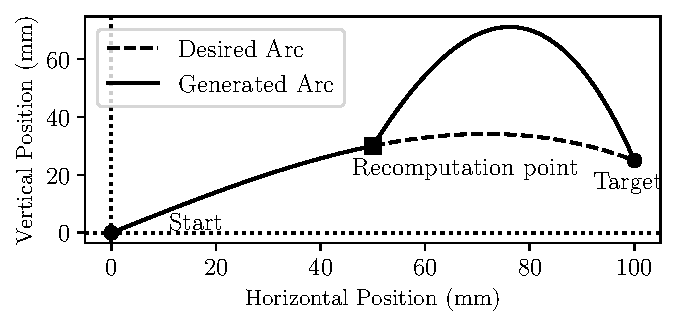
\includegraphics[clip, trim=0 0.25cm 0 0.25cm]{old_path.pdf}
                \caption{Existing arc recomputation problem}
                \label{fig:old_arc}
            \end{figure}

        \newpage
        \subsection{The Improved Trajectory System} \label{sec:imporved}
            The improved system solves this problem by utilising a flow function. During a step, this function will continuously calculate the
            direction that the foot must move to reach its destination. Thus this system is resilient to external disturbances and is capable of adjusting to
            varying destination and step height requirements. 
            
            The flow field is designed to first move the foot vertically upwards until horizontal coplanar with the destination, and then to follow a
            arc to the destination with a defined step height, this can be adjusted to make the arc start before or after coplanar. The step height can be adjusted at any point in time and the flow field will adjust accordingly.
            Figure \ref{fig:foot_arc} illustrates the field function and is described in section \ref{sec:flow_function}.
            \begin{figure}[h]
                \centering
                \hspace{-1.38cm}
                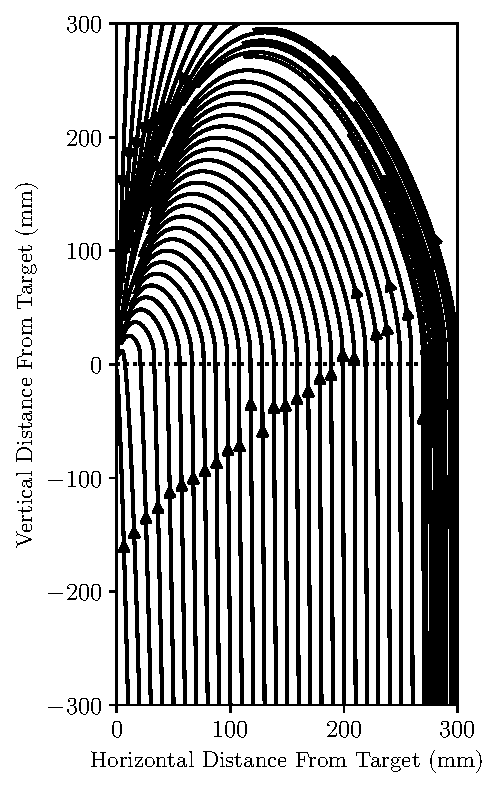
\includegraphics[clip, trim=0 0.25cm 0 0.25cm]{foot_path.pdf}
                \caption{End effector movement path}
                \label{fig:foot_arc}
            \end{figure}

            \subsubsection{Flow Function Description} \label{sec:flow_function}
                The flow function, \(\rho(x,y)\), uses the gradient function of a parabola passing through the point \([0,0]\) and \([x,y]\) as a basis, where point \([x,y]\)
                is the current point that is being evaluated and \(x\) is the horizontal distance between the destination and the current point and \(y\) the
                vertical distance. The final function is described by equations \ref{eq:rho} to \ref{eq:sigmoid}.
                \begin{equation} \label{eq:rho}
                    \begin{aligned}
                        \rho(x,y) &= \frac{\delta}{\delta x\delta y}&&f_a(x,y)x^2 + f_b(x,y)x + C\\
                        &= &&2f_a'(x,y)x + f_b'(x,y)    
                    \end{aligned}
                \end{equation}
                where, %\(f_a'(x,y)\) and \(f_b'(x,y)\) are defined as follows:
                \begin{align} \label{eq:fa}
                    f_a'(x,y) &= -\left|\frac{C_h}{x}\right| - \left|S(y)\right|\\
                    f_b'(x,y) &= \frac{y}{x} - f_a(x,y)
                \end{align}
                where \(C_h\) determines step height and \(S(y)\) is a sigmoid-like function responsible for the initial vertical rise. \(S(y)\) is defined in defined as
                \begin{equation} \label{eq:sigmoid}
                    S(y) = \frac{0.515(y-q)}{1+\left|y-q\right|-0.515}
                \end{equation}
                where \(q\) is the variable that determines at which vertical displacement the leg path transitions from primarily a vertical motion to an arc motion. Figure \ref{fig:sigmoid_like} illustrates the sigmoid-like function for different values of \(q\).
                \begin{figure}[h]
                    \centering
                    \hspace{-1.38cm}
                    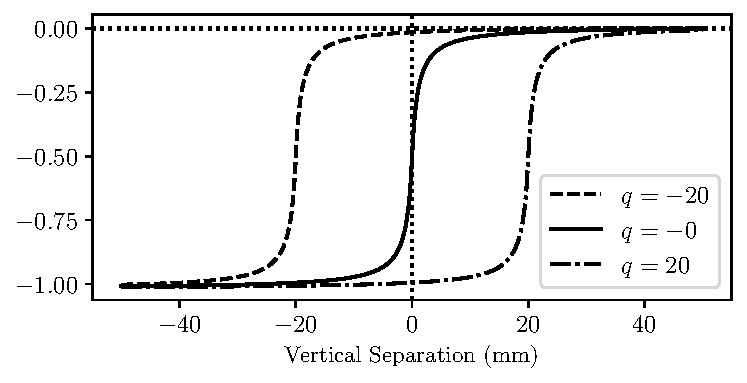
\includegraphics[clip, trim=0 0.25cm 0 0.25cm]{sigmoid_like.pdf}
                    \caption{Sigmoid Like}
                    \label{fig:sigmoid_like}
                \end{figure}

                \noindent
                Note that the 0.515 values in equation \ref{eq:sigmoid} are set to make its output range from roughly -1 to 0 over the active range.
                
                \newpage
                \subsubsection{Generated Trajectory Examples}
                To demonstrate the trajectories generated by the flow function, three different example are provided: One with the target on the same vertical level as the starting point, one with the target above the starting point, and one with the target below the starting point. Figures \ref{fig:traj1} to \ref{fig:traj3} show these three examples. Additionally, the parameters \(C_h\) and \(q\) are varied to show their effect. Please see \href{https://youtu.be/UfGo_LZfF2c}{\underline{this video}} for a simulated demonstration of the baseline walking system.
                \begin{figure}[h]
                    \centering
                    % \hspace{-1.38cm}
                    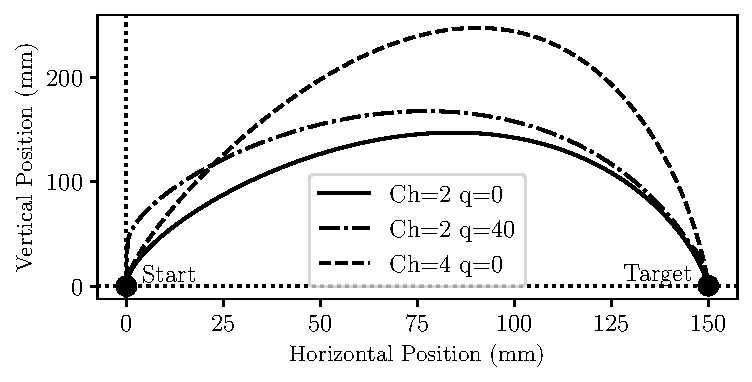
\includegraphics{traj_1.pdf}
                    \caption{Equal start and target example trajectories.}
                    \label{fig:traj1}
                \end{figure}

                \noindent
                As can be seen from figure \ref{fig:traj1} the parameter \(q\) specifies the initial vertical rise above the target position. When \(q\) is zero there is no additional vertical rise, similarly if q were to be made negative, the foot would start moving horizontally before the target's height is reached. While \(q\) does affect the stride height a little bit, the primary stride height parameter is \(C_h\). As can be seen from the figure, adjusting \(C_h\) drastically affects the stride height while leaving vertical rise above the target unaffected.

                The following example, shown in figure \ref{fig:traj2}, shows the trajectory for when the target is placed above the starting point. Here the initial vertical rise can be seen clearly. Note how increasing \(q\) lengthens the vertical rise. Importantly it can be seen that once the vertical rise is completed, the remaining arc is essentially equivalent to that in figure \ref{fig:traj1}. This is the intended benefit of using a policy such as the flow function.
                
                \begin{figure}[h]
                    \centering
                    % \hspace{-1.38cm}
                    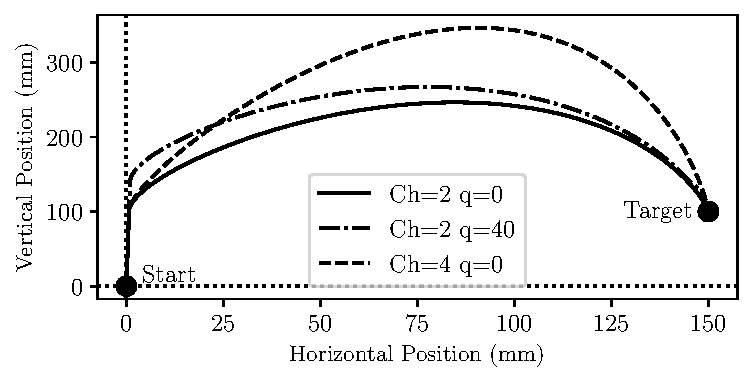
\includegraphics{traj_2.pdf}
                    \caption{Elevated target example trajectories.}
                    \label{fig:traj2}
                \end{figure}
                
                The next example is shown in figure \ref{fig:traj3}, this example has the target below the starting point. Here it can be seen that the generated trajectory has a much lower stride height compared to the previous examples. It should also be noted that in this case \(q\) has almost no effect on the resulting trajectory, this is because the starting point is already above the target, and thus the sigmoid governing the vertical rise is close to negligible.
                \begin{figure}[h]
                    \centering
                    % \hspace{-1.38cm}
                    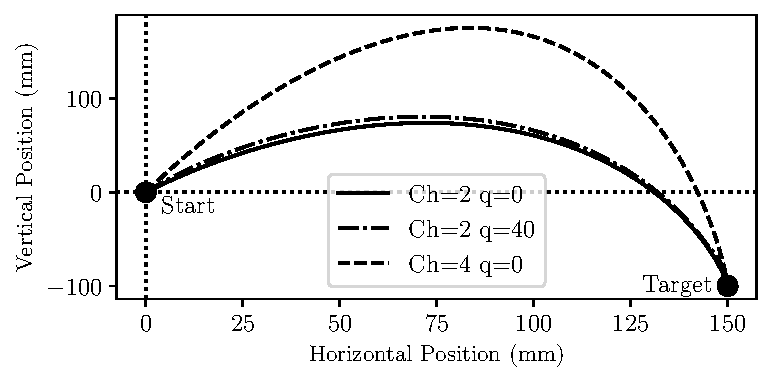
\includegraphics{traj_3.pdf}
                    \caption{Lowered target example trajectories.}
                    \label{fig:traj3}
                \end{figure}

                \noindent
                Next, two examples illustrating the recomputation capabilities provided by the flow function are shown. Figure \ref{fig:traj_re1} shows a similar initial setup to that in figure \ref{fig:traj_re1}, where the star and initial end positions are on the same vertical level. However, partway through the trajectory the target position is changed to be further away and below the starting point, indicated by the square marker. As can be seen, the flow function competently adjusts the stride length to reach the new target. Importantly, the overall stride height is essentially unchanged by this operation.
                \begin{figure}[h]
                    \centering
                    % \hspace{-1.38cm}
                    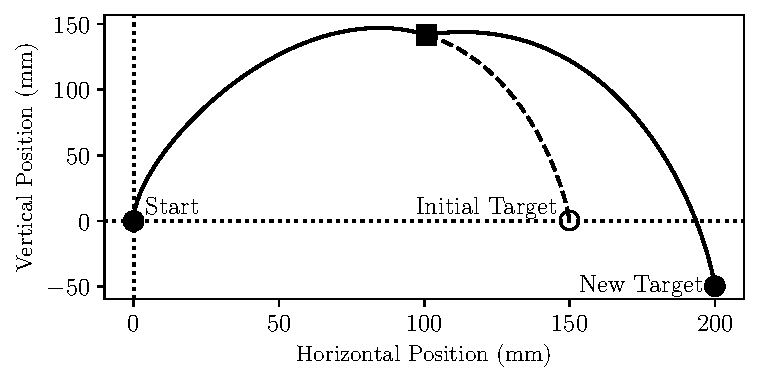
\includegraphics{traj_re1.pdf}
                    \caption{Recomputation example 1.}
                    \label{fig:traj_re1}
                \end{figure}

                \noindent
                In the second example, shown in figure \ref{fig:traj_re2}, the initial setup is equivalent to that in figure \ref{fig:traj3}, with the initial target below the start point. The target is then adjusted to be above and closer to the start. Similarly to the previous example, a competent new trajectory is generated. The stride length is shortened and the stride height remains mostly unchanged. It should be noted that there is no vertical rise as there was in figure \ref{fig:traj2}, this is because at the time the new target was provided, the foot was already above the new target.
                \begin{figure}[h]
                    \centering
                    % \hspace{-1.38cm}
                    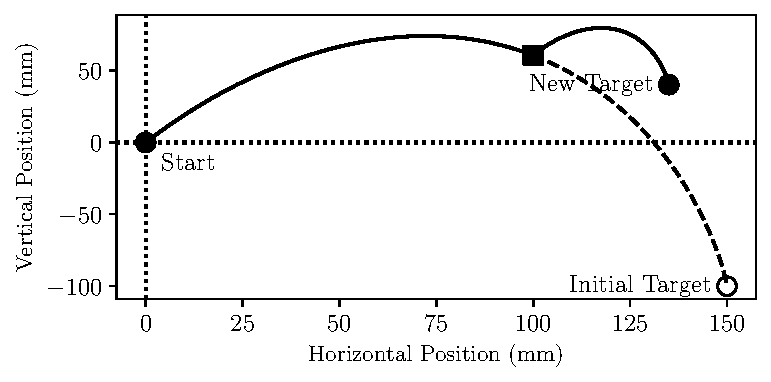
\includegraphics{traj_re2.pdf}
                    \caption{Recomputation example 2.}
                    \label{fig:traj_re2}
                \end{figure}
                
                